\chapter{Develop Code for Z-Way}
\label{c:developer}


\section{Z-Way software structure overview}

\begin{figure}
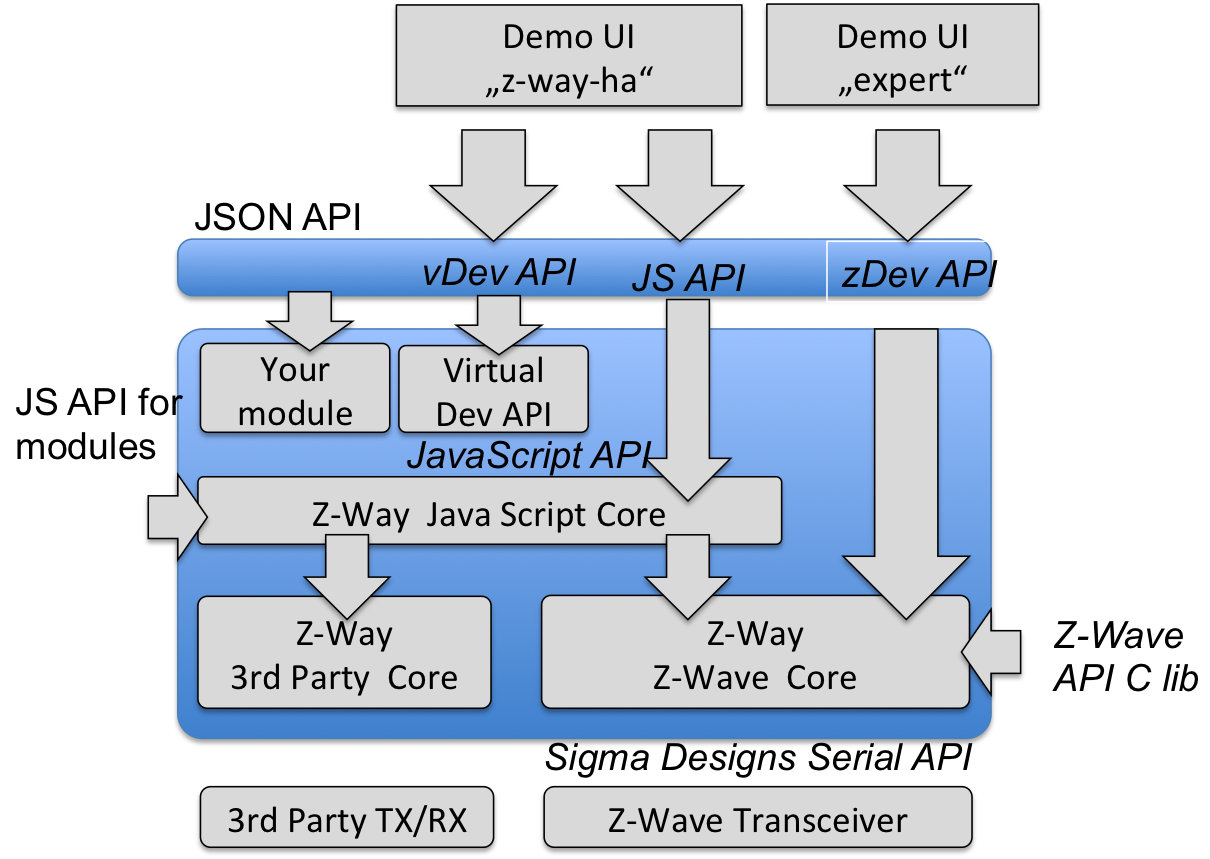
\includegraphics[width=0.9\textwidth]{pngs/cap11/apis.png}
\caption{Z-Way APIs and their use by GUI demos}
\label{apis}
\end{figure}

Z-Way offers multiple Application Program Interfaces (API) that are partly built on each 
other. Figure \ref{apis} shows the general structure of Z-Way with focus on the APIs. The 
most important part of Z-Way is the Z-Wave core. The Z-Wave core uses the standard Sigma 
Designs Serial API to communicate with a Z-Wave compatible transceiver hardware but enhanced 
with some Z-Way specific functions such as frequency change. The standard interface is 
not public but available for owners of the Sigma Designs Development Kit (SDK)
\footnote{The Sigma Designs SDK is available from Digikey (www.digikey.com). Depending 
on the hardware options chosen the price varies between 2000 and 4000 USD only.}

The Z-Wave core services can be accessed directly using the Z-Wave Device API (zDev API). 
There are two Z-Wave device API versions available:
\begin{itemize}
\item Z-Wave API as JSON API: All functions are available using a JSON API implemented 
by an embedded webserver. This web server can be used in two ways:
\begin{itemize}
\item web sockets, a permanent IP connection
\item REST (Representational State Transfer)
\end{itemize}
Both ways to use the JSON API have the same data structures and commands. The 
\zweui as described in chapter \ref{eui} uses the REST option of this JSON API. This user 
interface is a very good reference how to apply the Z-Wave Device API. For oore 
information about the Z-Wave Device API please refer to Section \ref{zwavedeviceapi}.

\item Z-Wave API as C Library API: All functions of the JSON API are available as C 
library function too. The URL

\murl{http://razberry.z-wave.me/fileadmin/z-way-test.tgz}

provides a sample application written in standard C that makes use of the C level 
API to demonstrate its application. Makefiles and project files for compilation on 
Linux and OSX are provided together with the sample code. More information on the C 
level API you find in Section \ref{clevelapi}.

\end{itemize}


The \textbf{Z-Wave device API only allows the management of the Z-Wave network} and 
the control and management of the devices as such. No higher order logic except the 
so-called Z-Wave associations between two Z-Wave devices can be used.

For all \textbf{automation and higher order logic a JavaScript automation engine} 
is available. This engine is also shipped with Z-Way.

The JavaScript API on top of the JS engine mirrors all functions of the Z-Wave Device API 
but also allows access to third-party  device APIs (e.g. EnOcean). This means the JS API 
is the common ground for all further application logic and user interfaces (with the 
exception of the \zweui that uses the Z-Wave Device API.

The JavaScript layer makes use of a JavaScript implementation provided by Google it 
is also used in Googles Chrome web browser. All JavaScript API functions can also be 
accessed using the embedded webserver. The beauty of this interface is that JavaScript 
can be executed on the server and on the client. Executing on the client makes sense 
for small changes to the data model or running small helper programs.

There are two important sub-portions of the JavaScript layer:

\begin{itemize}

\item Virtual Devices (vDevs): All functions of the physical devices plus other functions are 
mapped into virtual devices. Virtual devices have properties and attributes linked to 
their physical counterpart functions. The \zwshui is completely 
written using the virtual device concept and this user interface can act as a good reference 
how to use them. Please refer to chapter \ref{c2} for more information about the 
use of the vdev concept.

\item The Apps: These are JavaScript portions that are dynamically loaded into the JS 
core and implement application or user specific function. Please refer to chapter \ref{apps} 
for more information about the app concept and existing apps. Please refer to Chapter 
\ref{developownapps} for more information about how to develop own apps.

\end{itemize}

\section{Z-Way APIs Quick Reference}

\subsection{Z-Wave Device API}
\label{zwavedeviceapi}

The Z-Wave Device API implements the direct access to the Z-Wave network. All Z-Wave devices 
are referred to by their unique identification in the wireless network---the Node ID. 
Z-Wave devices may have different instances of the same function, also called channels 
(for example sockets in a power strip). The Z-Wave Device API refers to them as daughter 
objects of the physical device object identified by an instance ID. In case there is 
only one instance, the instance ID = 0 is used.

\subsubsection {Sending Z-Wave Commands}

All device variables and available commands in a Z-Wave device are grouped in the so-called 
command classes. The Z-Wave API allows direct access to all parameters, values and commands 
of these command class structures. Annex \ref{ccs} gives you the complete reference of 
the implemented command classes.

Beside the devices the Z-Wave Device API also offers access to the management interface of 
the network. Annex \ref{FunctionClasses} gives you a full reference of the implemented 
function classes.

The Z-Wave Device API can be accessed on the JSON API with any standard web browser using the URL

\murl{http://YOURIP:8083/ZWaveAPI/*}.

Device objects or commands of these objects are accessed by

\murl{http://YOURIP:8083/ZWaveAPI/Run/devices[*].* }

\murl{http://YOURIP:8083/ZWaveAPI/Run/devices[x].instances[y].*}

\textbf{http://YOURIP:8083/ZWaveAPI/Run/devices[x].instances[y].commandClasses[z].*}

The whole data tree of the Z-Wave network is accessed using


\murl{http://YOURIP:8083/ZWaveAPI/Data/*}.

Please refer to the \zway for information about the context, the 
commands, and the data used. Section \ref{c2} provides more information
about the API and the underlying data structure.

All acces ot the webserver require authentication of the user. Please refer to Chapter 
\ref{cap:authentication} for details how to authenticate.

\subsection{JavaScript API (JS API)}

The Z-Wave Device API or any other third-party technology API do not offer any higher order
logic support but the pure access to functions and parameters of devices only.

Z-Way offers an automation engine to overcome this restriction. A server-side JavaScript 
runtime environment allows writing JavaScript modules that are executed within Z-Way 
(means on the server). The same time all functions of the JS API can also be accessed on 
the client side (the web browser). This offers some cool debug and test capabilities. 
Among others it is possible to write whole JS functions right into the URL or the browser.

The JS API can be accessed from the web browser with the URL

\murl{http://YOURIP:8083/JS/Run/*}


Among others the whole Z-Wave Device API is available within the JS API using 
the object ``zway’‘. As a result, the following three statements refer to the very same function:

\begin{enumerate}
\item \textbf{http://YOURIP:8083/ZWaveAPI/Run/devices[3].*} Client Side URL access using the Z-Wave Device API.
\item \textbf{http://YOURIP:8083/JS/Run/zway.devices[3].*}: Client Side URL access using the JS API
\item \textbf{zway.devices[3].*}: Server Side access using the JS and the public zway object
\end{enumerate}

Due to the scripting nature of JavaScript it is possible to ``inject’‘ code at run time 
using the interface. Here a nice example how to use the JavaScript setInterval function:

\begin{lstlisting}[caption=Polling of device \#2]{Name}
/JS/Run/setInterval(function() {
	zway.devices[2].Basic.Get();
}, 300*1000);
\end{lstlisting}

This code will, once ``executed’‘ as URL within a web browser, call the Get() command
of the command class Basic of Node ID 2 every 300 seconds.

A very powerful function of the JS API is the ability to bind functions to certain values 
of the device tree. They get then executed when the value changes. Here is an example 
for this binding. The device No. 3 has a command class SensorMultilevel that offers 
the variable ``level.’’ The following call---both available on the client side and 
on the server side---will bind a simple alert function to the change of the variable.

\begin{lstlisting}[caption=Bind a function]{Name}
zway.devices[3].SensorMultilevel.data[1].val.bind( function() {
	debugPrint('CHANGED TO:' + this.value + '\n');
});
\end{lstlisting}

\footnote{Please note that the Sensor Multilevel Command class data is an array index 
by the scale ID. Other command classes such as Basic do not have this index but allow 
direct access using CommandClassName.data.level}

Chapter \ref{c2} and \ref{datamodel} describe the whole JS API in detail. The 
names and IDs of the different command classes as well as their instance variables 
can be found in the Annex \ref{ccs}.

JavaScript modules can and will generate new functions that are accessible using the 
JSON interface. For simplification function calls on the API (means on the client side) 
are written in URL style starting with the word ``ZAutomation’’:


\begin{center}
/ZAutomation/JSfunction/JParameter
== JSfunction(JParameter)
\end{center}

\subsection{Virtual Device API}

All functions and instances of a physical device, which are represented as daughter objects
in the Z-Wave Device API, are enrolled into individual virtual devices.

In case the Z-Wave API shows one single physical device with two channels, the Virtual 
Device API will show two devices with similar functionality. In case the Z-Wave API shows 
a physical device with several functions (like a binary switch and an analog sensor in 
one device), the Virtual Device API (vDev API) will show them as several devices with 
one function each.

The vDev is accessed using the JSON API in a slightly different style than zDev API. 
All devices, variables, and commands are encoded into a URL style for easier handling 
in AJAX code. A typical client-side command in the vDev API looks like


\murl{http://YOURIP:8083/ZAutomation/api/v1/devices/ZWayVDev\_6:0:37/command/off}


``API’’ points to the vDev API function, ``v1’’ is just a constant to allow future extensions. 
The devices are referred to by a name that is automatically generated from the Z-Wave Device 
API. The vDev also unifies the commands ``command’’ and the parameters, here ``off.’’

On the server side, the very same command would be encoded in a JavaScript style.

\begin{lstlisting}[caption=Bind a function]{Name}
	dev = this.controller.devices.get('ZWayVDev\_6:0:37');
	dev.command('off');
\end{lstlisting}

The vDev API also offers support for notifications, locations information, the use of other modules, etc.

\subsection{Comparison}

Table \ref{c1:comp} summarizes the functions of the different APIs.


\begin{table}
\begin{tabular}{|p{40mm}|p{50mm}|p{20mm}|p{20mm}|}
\hline
API Type &	Core Function & Network Management & Automation\\
\hline
Z-Wave Dev API (JSON)	& Access to physical network and physical devices via JSON	&
Yes	&No\\
\hline
Z-Wave Dev API (C lib) 	& Access to physical network and physical devices via C style calls &
Yes	&No\\
\hline
JavaScript API & Access to physical network and devices plus JS type functions	&
No	&Yes, via zDev\\
\hline
vDev API & Unified Access to functions of devices, optimized for AJAX GUI&
No	&Yes\\
\hline
\hline
\end{tabular}
\caption{Different APIs of the Z-Way system}
\label{c1:comp}
\end{table}		
